\documentclass[11pt,a4paper]{article}
\usepackage[margin={2.6cm,2.6cm}]{geometry}
\usepackage{lmodern}
\usepackage{microtype}
\usepackage{enumitem}
\usepackage{array}
\usepackage[spanish,es-tabla]{babel}
\usepackage[utf8]{inputenc}
\usepackage[T1]{fontenc}
\usepackage{amsmath, amsthm}
\usepackage{hyperref}
\usepackage{xcolor}
\usepackage{graphicx}
\usepackage{listings}
\usepackage{fontawesome5}
\usepackage{dirtree}


\definecolor{azuluc}{HTML}{1F4E79}
\definecolor{grisclaro}{HTML}{F4F6F8}
\definecolor{gris}{HTML}{586069}
\definecolor{verde}{HTML}{2E7D32}
\definecolor{rojo}{HTML}{A94442}
\definecolor{git}{HTML}{F1502F}

\definecolor{morado_ubuntu}{RGB}{48, 10, 36}       % Fondo morado oscuro de Ubuntu GNOME
\definecolor{verde_ubuntu}{RGB}{78, 154, 6}        % Verde para comentarios
\definecolor{cyan_ubuntu}{RGB}{52, 226, 226}       % Cian para comandos
\definecolor{amarillo_ubuntu}{RGB}{250, 240, 190}  % Amarillo para cadenas
\definecolor{rojo_ubuntu}{RGB}{220, 50, 47}        % Rojo para errores
\definecolor{verde_claro_ubuntu}{RGB}{138, 226, 52} % Verde claro para el prompt
\definecolor{azul_ubuntu}{RGB}{114, 159, 207}      % Azul para símbolos y rutas
\definecolor{gris_ubuntu}{RGB}{128, 128, 128}      % Gris para el borde del frame


\definecolor{fondo_mac}{RGB}{255, 255, 250}       % Fondo beige claro típico de macOS
\definecolor{negro}{RGB}{0, 0, 0}                 % Texto en negro
\definecolor{verde_mac}{RGB}{63, 127, 95}         % Verde para comentarios
\definecolor{azul_mac}{RGB}{0, 0, 255}            % Azul para comandos y prompt
\definecolor{rojo_mac}{RGB}{196, 26, 22}          % Rojo para errores y cadenas
\definecolor{morado_mac}{RGB}{147, 39, 143}       % Morado para emphasis (opcional)
\definecolor{gris_mac}{RGB}{200, 200, 200}        % Gris para el borde del frame



\lstdefinestyle{rstyle}{
  language=R,
  basicstyle=\ttfamily\small,
  keywordstyle=\color{azuluc}\bfseries,
  commentstyle=\color{gris},
  stringstyle=\color{verde!70!black},
  showstringspaces=false,
  frame=single,
  rulecolor=\color{gris!30},
  backgroundcolor=\color{grisclaro},
  breaklines=true,
  showspaces=false,
  tabsize=2
}

\lstdefinestyle{rconsole}{
  language=R,
  basicstyle=\color{rojo}\ttfamily\small,
  showstringspaces=false,
  columns=fullflexible,
  frame=single,
  rulecolor=\color{gris!30},
  breaklines=true,
  tabsize=2
}

\lstdefinestyle{routput}{
  language=R,
  basicstyle=\color{azuluc}\ttfamily\small,
  showstringspaces=false,
  columns=fullflexible,
  frame=single,
  rulecolor=\color{gris!30},
  breaklines=true,
  tabsize=2
}

\lstdefinestyle{mdstyle}{
  basicstyle=\ttfamily\small,
  keywordstyle=\color{azuluc}\bfseries,
  commentstyle=\color{gris},
  stringstyle=\color{verde!70!black},
  showstringspaces=false,
  showspaces=false,
  tabsize=2,
  frame=single,
  rulecolor=\color{gris!30},
  backgroundcolor=\color{grisclaro},
  breaklines=true,
  breakatwhitespace=false,
  % Reglas específicas para Markdown
  morekeywords={*,\#,-,[,],(,),!,`,~,.,=},
  % Títulos Markdown
  morecomment=[l][\color{azuluc}\bfseries]{\#},
  % Enlaces y referencias
  morecomment=[s][\color{rosa}]{[}{]},
  morecomment=[s][\color{verde}]{(}{)},
  % Cadenas
  morestring=[b][\color{naranja}]{"},
  morestring=[b][\color{naranja}]{'},
  % Lenguajes utilizados en bloques de código
  classoffset=1,
    keywordstyle=\color{morado}\bfseries,
    morekeywords={python,bash,R,latex,json,yaml},
  classoffset=0,
  % Protocolos y enlaces
  emph={http,https,ftp},
  emphstyle=\color{azuluc}\underbar,   
   literate=
    {á}{{\'a}}1
    {é}{{\'e}}1
    {í}{{\'i}}1
    {ó}{{\'o}}1
    {ú}{{\'u}}1
    {Á}{{\'A}}1
    {É}{{\'E}}1
    {Í}{{\'I}}1
    {Ó}{{\'O}}1
    {Ú}{{\'U}}1
    {ñ}{{\~n}}1
    {Ñ}{{\~N}}1
    {ü}{{\"u}}1
    {Ü}{{\"U}}1
}

\lstdefinestyle{ubuntugnome}{
  basicstyle=\ttfamily\small\color{white},
  backgroundcolor=\color{morado_ubuntu},
  commentstyle=\color{verde_ubuntu},
  keywordstyle=\color{cyan_ubuntu},
  stringstyle=\color{amarillo_ubuntu},
  emphstyle=\color{rojo_ubuntu},
  showstringspaces=false,
  frame=single,
  rulecolor=\color{gris_ubuntu},
  breaklines=true,
  postbreak=\mbox{\textcolor{white}{$\hookrightarrow$}\space},
  % Configuración para simular el prompt de Ubuntu
  upquote=true,
  % Resaltar el prompt de usuario
  emph={user@ubuntu:~\$},
  emphstyle={\color{verde_claro_ubuntu}\bfseries},
  % Resaltar errores (ej: "command not found")
  classoffset=1,
  emph={command not found,No such file or directory,Permission denied},
  emphstyle={\color{rojo_ubuntu}},
  classoffset=0,
}

\lstdefinestyle{macterminal}{
  basicstyle=\ttfamily\small\color{negro},
  backgroundcolor=\color{fondo_mac},
  commentstyle=\color{verde_mac},
  keywordstyle=\color{azul_mac},
  stringstyle=\color{rojo_mac},
  emphstyle=\color{morado_mac},
  showstringspaces=false,
  frame=single,
  rulecolor=\color{gris_mac},
  breaklines=true,
  postbreak=\mbox{\textcolor{negro}{$\hookrightarrow$}\space},
  % Configuración para simular el prompt de macOS
  upquote=true,
  % Resaltar el prompt de usuario
  emphstyle={\color{azul_mac}\bfseries},
  % Resaltar errores (ej: "command not found")
  classoffset=1,
  emph={command not found,No such file or directory,Permission denied},
  emphstyle={\color{rojo_mac}},
  classoffset=0
}

\lstdefinestyle{windowscmd}{
  basicstyle=\ttfamily\small\color{white},
  backgroundcolor=\color{black},
  showstringspaces=false,
  frame=single,
  rulecolor=\color{gris_mac},
  breaklines=true,
  postbreak=\mbox{\textcolor{negro}{$\hookrightarrow$}\space},
  % Configuración para simular el prompt de macOS
  upquote=true,
  % Resaltar el prompt de usuario
  emphstyle={\color{azul_mac}\bfseries},
  % Resaltar errores (ej: "command not found")
  classoffset=1,
  emph={command not found,No such file or directory,Permission denied},
  emphstyle={\color{rojo_mac}},
  classoffset=0
}



\newcommand{\R}{\textcolor{azuluc}{\faIcon{r-project}}}
\newcommand{\Git}{\textcolor{git}{\faIcon{git-alt}}~\!Git}
\newcommand{\GitHub}{\faIcon{github}~\!GitHub}

\newtheoremstyle{exercise}
  {0.8em}{0.8em}{\normalfont}{}{\bfseries\color{azuluc}}{.}{0.5em}{}
\theoremstyle{exercise}
\newtheorem{exercise}{Ejercicio}


\title{\LARGE \textbf{Práctica 2: Introducción a \Git\ y a \GitHub} \\[0.5em]
\Large Laboratorio de Matemáticas \\
\small \ \\
Grado en Ingeniería Matemática - Doble Grado en Física e Ingeniería Matemática}
\author{Miguel Beltra Vidal}
\date{Curso 2026/27}

\begin{document}

\maketitle

\section{Objetivos}

El objetivo de esta práctica es introducir el sistema de control de versión \Git\ y la plataforma de desarrollo colaborativo \GitHub. Al finalizarla, el estudiante será capaz de llevar un control de las diferentes versiones de sus proyectos y podrá almacenarlos en \GitHub.

\section{Sistemas de control de versiones}

Por sistema de control de versiones se entiende un programa que es capaz de llevar un registro de las diferentes versiones de un proyecto, indicando qué cambios han sucedido: qué ficheros se han añadido, qué ficheros se han borrado o qué cambios se han producido en un fichero, entre otras cosas. Existen numerosos sistemas de control de versiones, como pueden ser Subversion, Mercurial o Perforce, pero en esta asignatura introduciremos \Git, por ser el más popular y de código abierto. De acuerdo con la documentación oficial:

\medskip

\begin{center}
\begin{minipage}{0.8\linewidth}
	\emph{Git es un sistema de control de versiones distribuido, gratuito y de código abierto, diseñado para gestionar desde proyectos pequeños hasta proyectos de gran envergadura con rapidez y eficiencia.}
\end{minipage}
\end{center}


\subsection{Plataformas de desarrollo colaborativo}

Una plataforma de desarrollo colaborativo (también llamada Forja) es una plataforma que permite que albergar proyectos para que las personas puedan trabajar en ellos. \GitHub\ es una plataforma de este tipo que permite alojar proyectos utilizando \Git.



\section[Primeros pasos con Git]{Primeros pasos con \Git}


\subsection[Instalación de Git]{Instalación de \Git}

\subsubsection{Instalación en Linux}

Para instalar \Git\ en Linux, seguiremos el procedimiento habitual. Por ejemplo, si nuestra distribución es Ubuntu, entonces ejecutaremos los comandos siguientes en la consola:
\begin{lstlisting}[style=ubuntugnome]
$ sudo apt update
$ sudo apt install git
\end{lstlisting}
Comprobaremos que se ha instalado con el comando:
\begin{lstlisting}[style=ubuntugnome]
$ git --version
\end{lstlisting}
Nos debería dar información acerca de la versión de \Git\ que hemos instalado.


\subsubsection{Instalación en MacOS}

\Git\ viene incluido con las Xcode Command Line Tools, que son herramientas de desarrollo esenciales para macOS. Abre la Terminal (puedes buscarla en Spotlight con \texttt{Cmd + Espacio} y escribir \texttt{Terminal}). Ejecuta el siguiente comando para instalar las Xcode Command Line Tools:

\begin{lstlisting}[style=macterminal]
xcode-select --install
\end{lstlisting}

\noindent Una vez instalada, puedes ver que efectivamente se ha instalado con el comando siguiente:

\begin{lstlisting}[style=macterminal]
git --version
\end{lstlisting}


\subsubsection{Instalación en Windows}

Entramos en la web oficial: \url{https://git-scm.com/}. Desde aquí podemos descargar el instalador. Para este curso será suficiente con marcar las opciones de configuración sugeridas por el instalador.

\begin{center}
	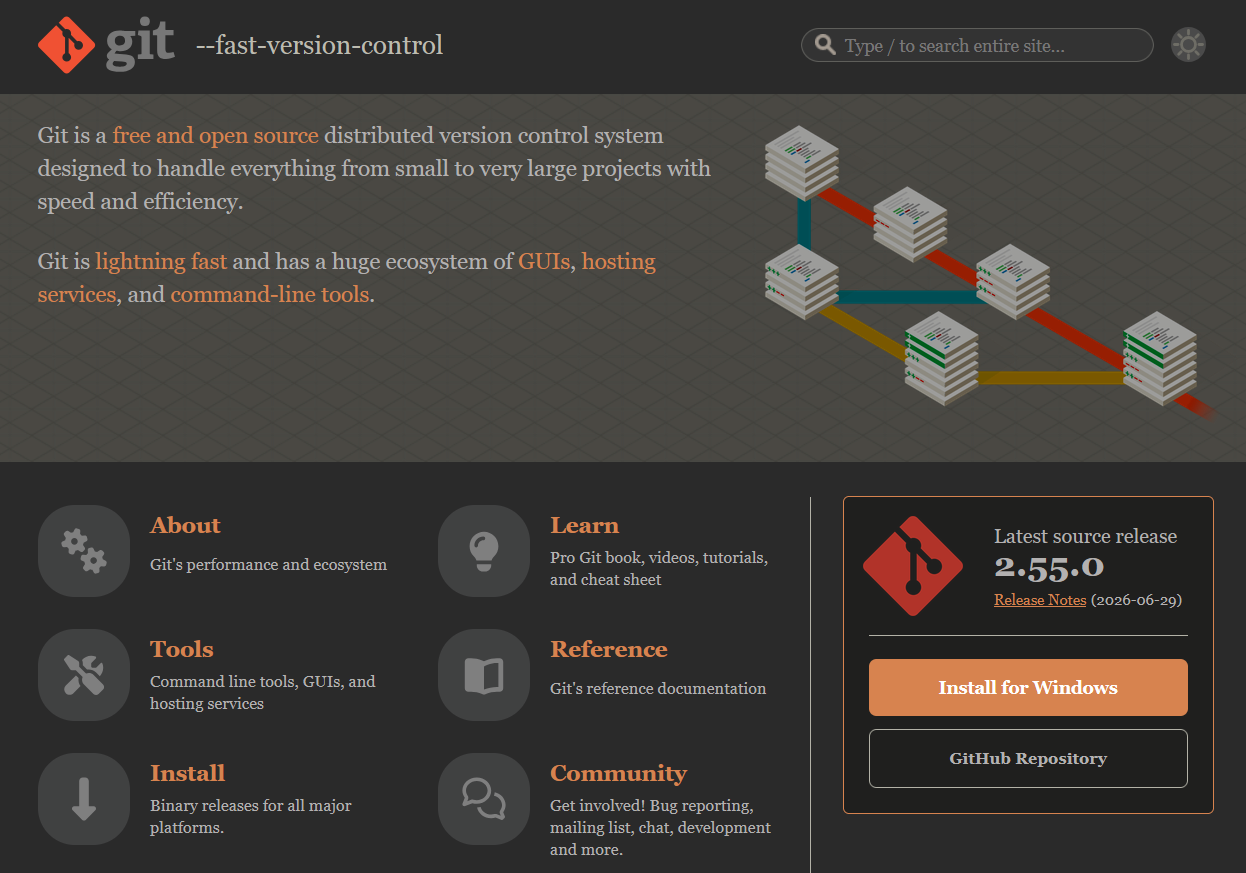
\includegraphics[scale=.4]{images/git_web.png}
\end{center}

\noindent Podemos comprobar que se ha instalado correctamente desde la consola de comandos \texttt{cmd} de Windows ejecutando el comando:

\begin{lstlisting}[style=windowscmd]
C:\Users\user> git --version
\end{lstlisting}


\subsection[Configuración de usuario en Git]{Configuración de usuario en \Git}


Configuraremos nuestro usuario de \Git\ con los siguientes comandos:
\begin{lstlisting}[style=ubuntugnome]
git config --global user.name "Tu Nombre"
git config --global user.email "tu.email@example.com"
\end{lstlisting}


\subsection{Primer proyecto y primeros comandos}

En la consola de comandos de nuestro sistema operativo nos situaremos en el directorio que contendrá el código de nuestras prácticas, y ejecutaremos el siguiente comando para iniciar nuestro repositorio de \Git:

\begin{lstlisting}[style=ubuntugnome]
git init
\end{lstlisting}

A continuación, crearemos un directorio que contendrá los ficheros con los que trabajaremos en nuestra práctica. Por ejemplo, añade a la estructura de directorios de la práctica 1 un nuevo directorio que se llame \texttt{Git}. Dentro de este, crearemos un fichero llamado \texttt{README.md}. Con tu editor de texto de preferencia, escribe en él algo como lo siguiente:

\medskip

\begin{lstlisting}[style=mdstyle]
# Práctica de Git y GitHub

*Autor:* Miguel Beltrá Vidal
\end{lstlisting}

El fichero de texto que acabamos de crear es de tipo \texttt{Markdown}. Estos ficheros tienen la extensión \texttt{.md} y suelen utilizar para escribir ficheros de documentación, como pueden ser los habituales \texttt{README.md} que se encuentran en la mayoría de proyectos. En una práctica futura estudiaremos \texttt{Markdown}. Por el momento, es suficiente con imitar el estilo de los ejemplos de esta práctica.

La estructura de directorios debería quedar algo así:

\begin{center}
\begin{minipage}{0.75\linewidth}
\dirtree{%
    .1 \faIcon[regular]{folder-open}\ practicas/.
	    .2 \faIcon[regular]{folder-open}\ .git/.
        .2 \faIcon[regular]{folder-open}\ Git/.
            .3 \faIcon[regular]{file-alt}\ README.md.
        .2 \faIcon[regular]{folder-open}\ R/.
            .3 \faIcon[regular]{folder-open}\ practica\_1/.
                .4 \faIcon[regular]{file-alt}\ ej1.R.
                .4 \faIcon[regular]{file-alt}\ ej2.R.
                .4 \faIcon[regular]{file-alt}\ ej3.R.
            .3 ....
}
\end{minipage}
\end{center}

Es posible que no veas el directorio \texttt{.git}. Esto se debe a que, como norma general, directorios y ficheros que empiezan por un punto (\texttt{.}) se interpretan como ficheros ocultos y el explorador de archivos en su configuración por defecto no los muestra. No pasa nada, ya que éste directorio contiene los ficheros necesarios para el control de versiones de \Git\ y nosotros no necesitaremos editarlos. Una vez creado nuestro repositorio de \Git\ y añadido el fichero  \texttt{README.md}, ejecutaremos el siguiente comando en la terminal:

\begin{lstlisting}[style=ubuntugnome]
git status
\end{lstlisting}

\noindent Nuestra salida debería ser similar a la siguiente:

\begin{lstlisting}[style=ubuntugnome,escapeinside={(*@}{@*)}]
On branch master

No commits yet

Untracked files:
  (use "git add <file>..." to include in what will be committed)
        (*@\color{red}{Git/}@*)
        (*@\color{red}{R/}@*)

nothing added to commit but untracked files present (use "git add" to track)
\end{lstlisting}

\noindent Como puedes observar, se resalta en color rojo como fichero sin seguimiento el fichero \texttt{README.md}. Esto quiere decir que ese fichero no forma parte de los ficheros cuyas versiones queremos controlar. Cuando subamos nuestros archivos a \GitHub, cosa que explicaremos más adelante, estos ficheros no se subirán. Para añadirlo a la lista de ficheros a seguir, emplearemos el comando \texttt{git add [nombre\_del\_fichero]}. Añadiremos este fichero y comprobaremos el estado del repositorio de \Git:

\begin{lstlisting}[style=ubuntugnome]
git add Git/README.md
git status
\end{lstlisting}

\noindent Nuestra salida debería ser similar a la siguiente:

\begin{lstlisting}[style=ubuntugnome,escapeinside={(*@}{@*)}]
On branch master

No commits yet

Changes to be committed:
  (use "git rm --cached <file>..." to unstage)
        (*@\color{green}{new file:   Git/README.md}@*)

Untracked files:
  (use "git add <file>..." to include in what will be committed)
        (*@\color{red}{R/}@*)
\end{lstlisting}

Ahora ya sabemos que tenemos un nuevo archivo en seguimiento. Para confirmar los cambios, deberemos ejecutar el comando:
\begin{center}
\texttt{git commit -m ``Mensaje con la informacion de los cambios''}. 
\end{center}
En nuestro caso, podemos hacer lo siguiente:
\begin{lstlisting}[style=ubuntugnome]
git commit -m "Initial commit"
\end{lstlisting}
Tras ejecutar este comando, obtendremos la siguiente salida, confirmando los cambios:
\begin{lstlisting}[style=ubuntugnome,escapeinside={(*@}{@*)}]
[master (root-commit) ec3a5e4] Initial commit
 1 file changed, 6 insertions(+)
 create mode 100644 Git/README.md
\end{lstlisting}
Si ahora miramos el estado del repositorio, con \texttt{git status}, podemos ver que no existe ningún cambio que deba ser confirmado, aunque seguimos con ficheros sin seguimiento.
\begin{lstlisting}[style=ubuntugnome,escapeinside={(*@}{@*)}]
On branch master
Untracked files:
  (use "git add <file>..." to include in what will be committed)
        (*@\color{red}{R/}@*)

nothing added to commit but untracked files present (use "git add" to track)
\end{lstlisting}
Realizaremos ahora un cambio en nuestro fichero \texttt{README.md}, añadiendo algo más de información. Por ejemplo:
\begin{lstlisting}[style=mdstyle]
# Práctica de Git y GitHub

*Autor:* Miguel Beltrá Vidal

## Descripción de la práctica

Este directorio lo utilizaremos para aprender los fundamentos de Git.
\end{lstlisting}

\noindent Si guardamos el fichero editado y ejecutamos: \begin{lstlisting}[style=ubuntugnome]
git status
\end{lstlisting}

\noindent Nuestra salida debería ser similar a la siguiente:

\begin{lstlisting}[style=ubuntugnome,escapeinside={(*@}{@*)}]
On branch master
Changes not staged for commit:
  (use "git add <file>..." to update what will be committed)
  (use "git restore <file>..." to discard changes in working directory)
        (*@\color{red}{modified:   Git/README.md}@*)

Untracked files:
  (use "git add <file>..." to include in what will be committed)
        (*@\color{red}{R/}@*)

no changes added to commit (use "git add" and/or "git commit -a")
\end{lstlisting}
Se nos informa que el fichero \texttt{README.md}, que está bajo seguimiento, ha sufrido alguna modificación. Lo añadimos al repositorio.
\begin{lstlisting}[style=ubuntugnome]
git add Git/README.md
git status
\end{lstlisting}
Y nos aparecerá que todos los cambios se han añadido:
\begin{lstlisting}[style=ubuntugnome,escapeinside={(*@}{@*)}]
On branch master
Changes to be committed:
  (use "git restore --staged <file>..." to unstage)
        (*@\color{green}{modified:   Git/README.md}@*)
        
Untracked files:
  (use "git add <file>..." to include in what will be committed)
        (*@\color{red}{R/}@*)
\end{lstlisting}
Finalmente, confirmaremos la modificación utilizando de nuevo el comando \texttt{git commit}:
\begin{lstlisting}[style=ubuntugnome]
git commit -m "Update Git/README.md"
\end{lstlisting}
Obtendremos la siguiente confirmación de cambios:
\begin{lstlisting}[style=ubuntugnome]
[master 2dd4ae5] Update Git/README.md
 1 file changed, 8 insertions(+)
\end{lstlisting}



\begin{exercise} Crea un fichero de \R\ llamado \texttt{prueba.R} con el siguiente código (es posible que ya lo tengas de una clase anterior. Si ese es el caso, entonces puedes moverlo al directorio \texttt{Git}):

\begin{lstlisting}[style=rstyle]
area_rectangulo <- function(base, altura) {
	base * altura
}

volumen_esfera <- function(radio) {
	4 / 3 * pi * radio^3
}

f <- function(x, y, z) {
	x^2 + x*y + y^2 + y*z + z^2 + x*z
}

area_rectangulo(3, 5)
volumen_esfera(2)
f(2,0,1)
\end{lstlisting}

\noindent Añadelo a \Git\ y confirma su adición con un mensaje explicativo, como puede ser \texttt{``Add prueba.R''}. A continuación añade las siguientes líneas de código al final del fichero:

\begin{lstlisting}[style=rstyle]
area_triangulo <- function(base, altura) {
	base * altura / 2
}

area_triangulo(4, 3)
\end{lstlisting}

\noindent Guárda los cambios, añádelos al repositorio de \Git\ y confirma los cambios con un mensaje tipo \texttt{``Update prueba.R''}.
\end{exercise}


\subsection{El fichero \texttt{.gitignore}}

Hay veces que en nuestro directorio tenemos ficheros de los cuales no queremos hacer un control de versiones ni guardarlos. Suelen ser ficheros que contienen datos sensibles (contraseñas o información personal), datos de configuración (propios de cada ordenador) o compilados, ya que con los ficheros de código podremos obtener el compilado cuando lo necesitamos. El fichero \texttt{.gitignore} lista todos aquellos ficheros que queremos ignorar para no llevar ningún control de versiones sobre ellos. En este apartado trataremos de entender el fichero \texttt{.gitignore}. 

Crearemos un fichero en nuestro directorio, que podemos llamar \texttt{fichero\_a\_ignorar.txt}. Lo editamos, escribiendo algo como:
\begin{lstlisting}[style=mdstyle]
Fichero que Git ignorará
\end{lstlisting}
\Git\ verá dicho fichero. Si ejecutamos:
\begin{lstlisting}[style=ubuntugnome]
git status
\end{lstlisting}
Veremos el fichero que hemos añadido.
\begin{lstlisting}[style=ubuntugnome,escapeinside={(*@}{@*)}]
On branch master
Untracked files:
  (use "git add <file>..." to include in what will be committed)
        (*@\color{red}{Git/fichero\_a\_ignorar.txt}@*)
        (*@\color{red}{R/}@*)

nothing added to commit but untracked files present (use "git add" to track)
\end{lstlisting}
Para evitar que Git tenga en cuenta el fichero, crearemos el fichero \texttt{.gitignore} en la raíz del repositorio (esto es, donde está el directorio \texttt{.git}), y en él escribiremos:
\begin{lstlisting}[style=mdstyle]
Git/fichero_a_ignorar.txt
\end{lstlisting}
Guardamos. Si volvemos a comprobar el estado:
\begin{lstlisting}[style=ubuntugnome]
git status
\end{lstlisting}
Veremos el fichero que hemos añadido es ignorado por \Git. 
Por el contrario, aparecerá el fichero \texttt{.gitignore} como fichero sin seguimiento.
\begin{lstlisting}[style=ubuntugnome,escapeinside={(*@}{@*)}]
On branch master
Untracked files:
  (use "git add <file>..." to include in what will be committed)
        (*@\color{red}{.gitignore}@*)
        (*@\color{red}{R/}@*)
        
nothing added to commit but untracked files present (use "git add" to track)
\end{lstlisting}

\noindent La estructura de nuestro directorio de prácticas debería ser parecida a la siguiente:

\begin{center}
\begin{minipage}{0.75\linewidth}
\dirtree{%
    .1 \faIcon[regular]{folder-open}\ practicas/.
	    .2 \faIcon[regular]{folder-open}\ .git/.
        .2 \faIcon[regular]{folder-open}\ Git/.
            .3 \faIcon[regular]{file-alt}\ fichero\_a\_ignorar.txt.
            .3 \faIcon[regular]{file-alt}\ prueba.R.
            .3 \faIcon[regular]{file-alt}\ README.md.
        .2 \faIcon[regular]{folder-open}\ R/.
            .3 \faIcon[regular]{folder-open}\ practica\_1/.
                .4 \faIcon[regular]{file-alt}\ ej1.R.
                .4 \faIcon[regular]{file-alt}\ ej2.R.
                .4 \faIcon[regular]{file-alt}\ ej3.R.
            .3 ....
        .2 \faIcon[regular]{file-alt}\ .gitignore.
}
\end{minipage}
\end{center}



\begin{exercise} Añade el fichero \texttt{.gitignore} al seguimiento de versiones. Realiza una confirmación con un mensaje explicativo, p. ej. \texttt{``Add .gitinore file''}.
\end{exercise}

\subsection{Añadir todos los ficheros con \texttt{git add .}}

Recuerda que si modificamos el fichero \texttt{README.md} del directorio \texttt{Git} y lo queremos añadir al repositorio, podemos utilizar el comando \texttt{git add Git/README.md}. Si tuvieramos muchos ficheros, entonces tendríamos que ir uno por uno. Si queremos añadir todos los ficheros al mismo tiempo, entonces utilizamos:
\begin{center}
\texttt{git add .}
\end{center}
\textbf{Es muy importante haber incluido en el \texttt{.gitignore} los ficheros de los que no queremos llevar un seguimiento.} De lo contrario, al ejecutar el comando \texttt{git add .} incluiremos todos ellos también.

\begin{exercise} Añade uno de los ficheros de la Práctica 1 al control de versiones, por ejemplo, el que tiene el ejercicio 1, y confirma añadiendo un mensaje explicativo. A continuación, añade todos los ficheros de la Práctica 1 que tengas hasta el momento. Ees posible que aun no hayas completado la Práctica 1 al momento de hacer este ejercicio. No pasa nada. A medida que vayas completando el trabajo, añade los cambios y confírmalos como hemos explicado en esta práctica.
\end{exercise}







\section[Uso de GitHub]{Uso de \GitHub}

\subsection{Registro en GitHub}

Lo primero que deberemos hacer es registrarnos en la plataforma GitHub.


\begin{center}
	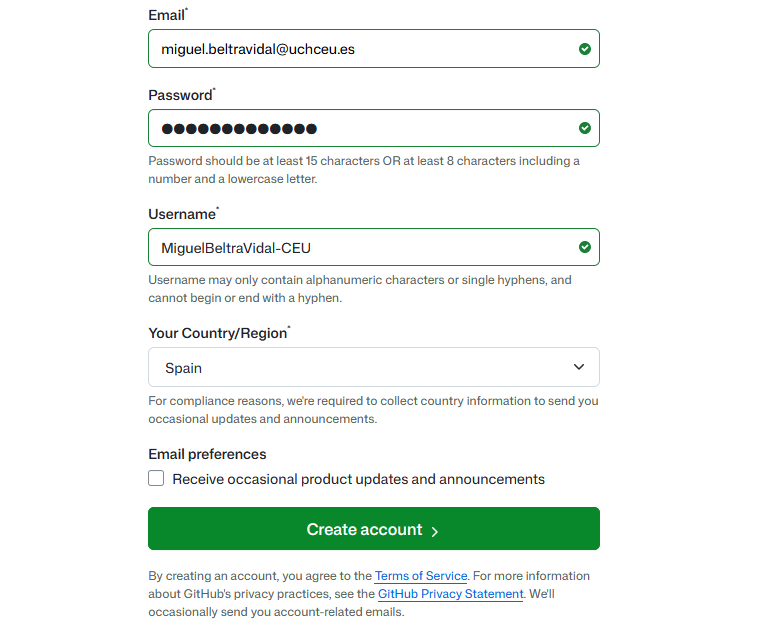
\includegraphics[scale=0.75]{images/registro_GitHub.png}
\end{center}

\subsection{Crear un nuevo repositorio}

Desde la vista principal de \GitHub\ podrás crear un nuevo repositorio con el botón \texttt{Create repository}:
\begin{center}
	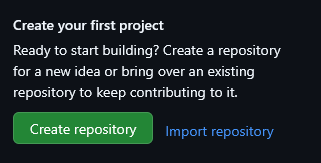
\includegraphics[scale=1]{images/primer_repositorio.png}
\end{center}
o clickando en \texttt{New} si ya tienes alguno creado:
\begin{center}
	
\includegraphics[scale=1]{images/nuevo_repositorio.png}
\end{center}

\noindent Pondremos un nombre al repositorio y lo marcaremos como privado.
\begin{center}
	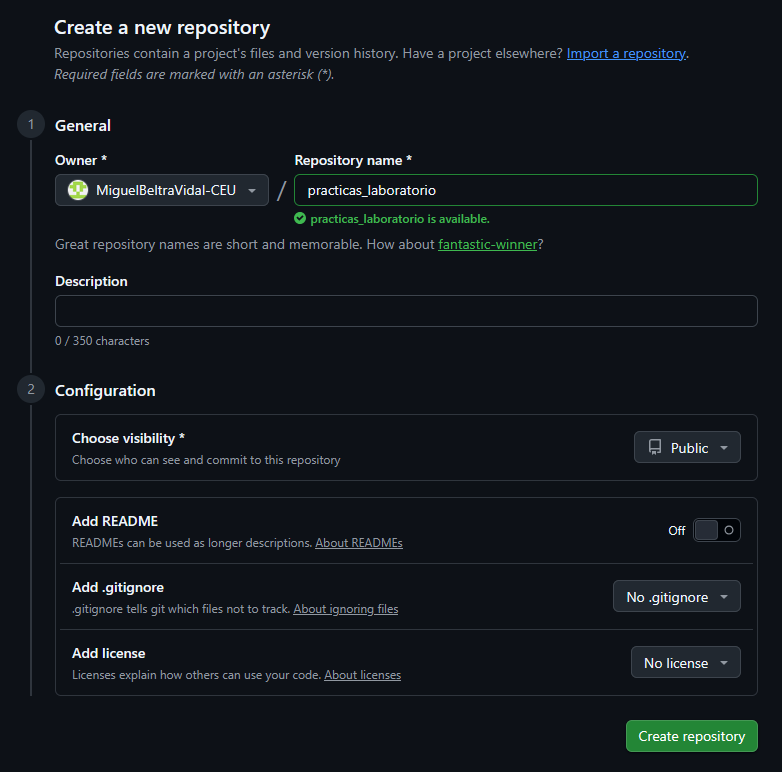
\includegraphics[scale=0.8]{images/nuevo_repositorio_2.png}
\end{center}

\noindent Invitaremos a un colaborador, en este caso, al profesor de la asignatura (\texttt{MiguelBeltraVidal-CEU}):
\begin{center}
	
\includegraphics[scale=0.8]{images/nuevo_repositorio_3.png}
\end{center}
\begin{center}
	
\includegraphics[scale=0.7]{images/nuevo_repositorio_4.png}
\end{center}
\begin{center}
	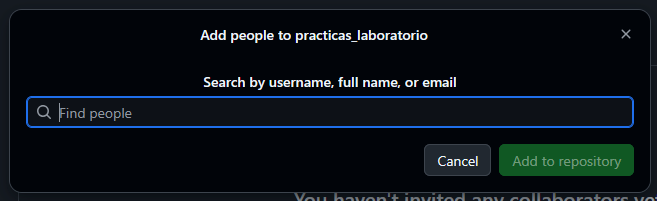
\includegraphics[scale=0.8]{images/nuevo_repositorio_5.png}
\end{center}

\noindent Podremos subir nuestro trabajo. Desde la vista principal de nuestro aparecen varias opciones para subir nuestro trabajo.
\begin{center}
	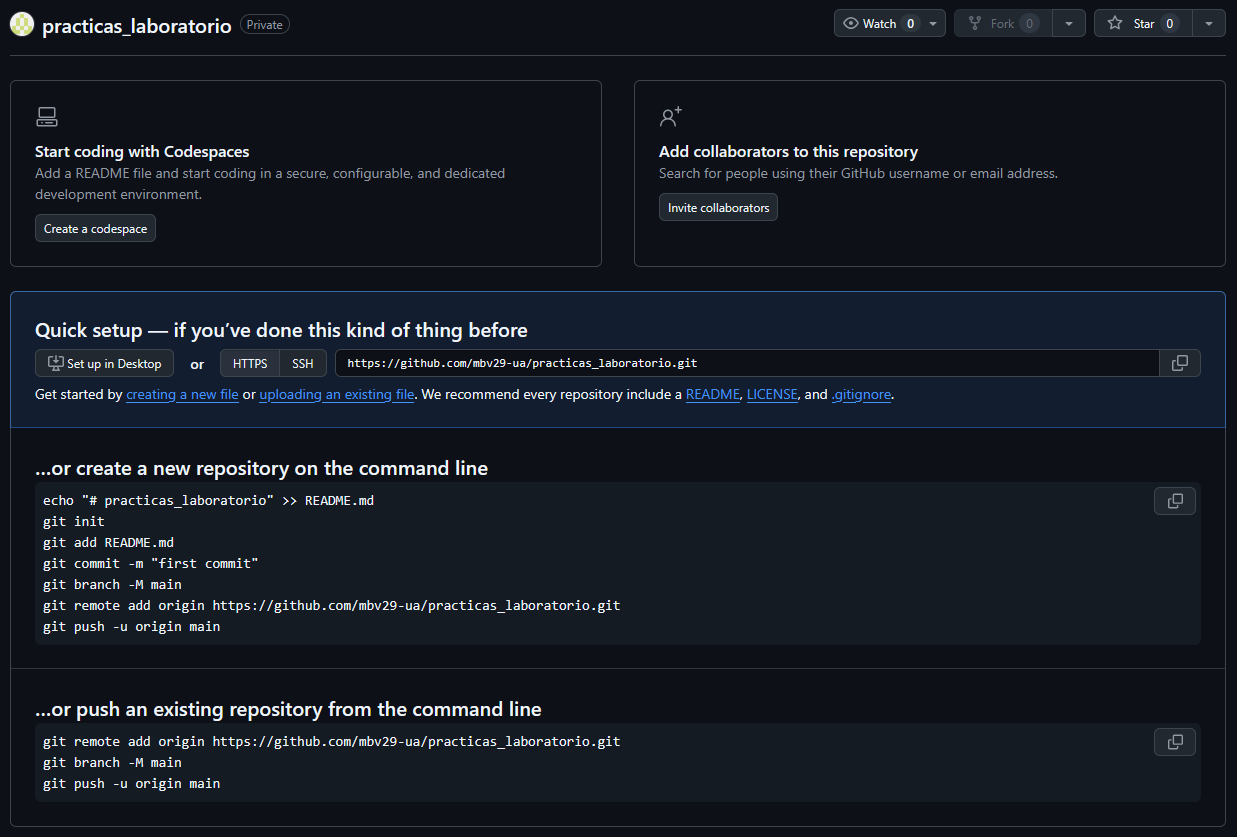
\includegraphics[scale=0.6]{images/nuevo_repositorio_6.png}
\end{center}

Como queremos subir un repositorio que ya existe en nuestro ordenador, nos fijaremos en la de abajo que tiene los comandos siguientes:
\begin{lstlisting}[style=ubuntugnome]
git remote add origin https://github.com/nombre_usuario/practicas_laboratorio.git
git branch -M main
git push -u origin main
\end{lstlisting}
Copiamos esos comandos desde GitHub y los ejecutamos en la terminal. El primer comando sirve para que nuestro repositorio local (el de nuestro ordenador) conozca el repositorio externo (el de \GitHub). El segundo hace un renombrado de nuestra rama (de momento no trabajaremos con varias ramas). El último comando es el que permite subir los cambios a \GitHub. Nos pedirá que autoricemos al gestor de credenciales, y ya lo tendremos.

\begin{center}
	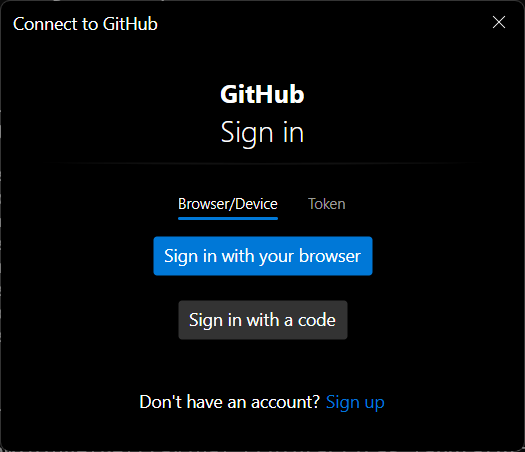
\includegraphics[scale=0.75]{images/autorizar_GitHub_1.png}
\end{center}
\begin{center}
	
\includegraphics[scale=0.6]{images/autorizar_GitHub_2.png}
\end{center}

\noindent Con esto, ya tendríamos nuestros ficheros subidos en \GitHub.

\begin{center}
	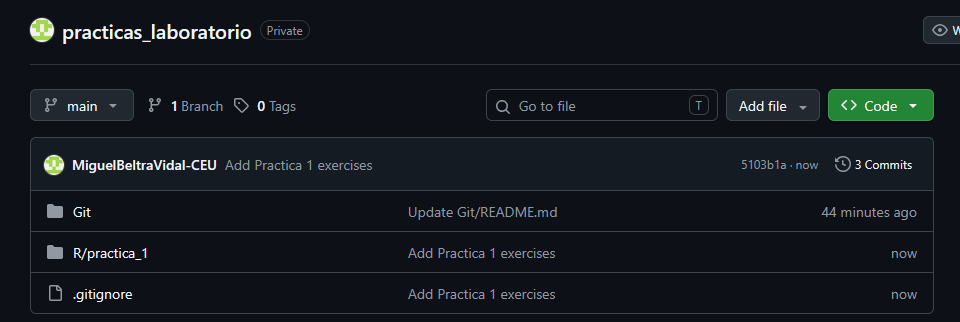
\includegraphics[scale=0.75]{images/comprobacion.png}
\end{center}



\section{Entrega y consejos}

Asegúrate de invitar al profesor a tu repositorio de prácticas para que pueda ver que las estás haciendo. Asegúrate de que en \GitHub\ aparezcan las últimas versiones de tus códigos. Deberás subir todos los ejercicios de la Práctica 1.

El flujo de trabajo habitual deberá ser el siguiente:

\paragraph{Antes de empezar}

\begin{enumerate}
\item Si tu ordenador no tiene \Git, instálalo y configura tu usuario.

\item Una vez tienes \Git:
\begin{enumerate}
\item Si en tu ordenador no tienes tus ficheros, clona tu repositorio de \GitHub\ con
\begin{lstlisting}[style=ubuntugnome]
git clone [direccion_del_repositorio]
\end{lstlisting}
Desde la página de tu repositorio de \GitHub\ puedes los detalles del \texttt{git clone} que vas a ejecutar.

\item Si en tu ordenador tienes una versión antigua de los ficheros, traete de \GitHub\ la última versión con el comando 
\begin{lstlisting}[style=ubuntugnome]
git pull
\end{lstlisting}
\end{enumerate}
\end{enumerate}



\paragraph{Durante tu sesión de trabajo}

\begin{enumerate}
\item Cada poco tiempo, cada vez que hagas un cambio importante, añadelo al repositorio con
\begin{lstlisting}[style=ubuntugnome]
git add [nombre_fichero]
\end{lstlisting}
o, si quieres añadir todos los cambios, con
\begin{lstlisting}[style=ubuntugnome]
git add .
\end{lstlisting}

	
\item Confirma los cambios con:
\begin{lstlisting}[style=ubuntugnome]
git commit -m "Comentario explicativo de los cambios"
\end{lstlisting}
	
\item Súbelos a \GitHub\ con:
	
\begin{lstlisting}[style=ubuntugnome]
git push
\end{lstlisting}
\end{enumerate}



\end{document}